\documentclass[a4paper, 12pt]{article}

\usepackage[english]{babel}
\usepackage[utf8]{inputenc}
\usepackage [autostyle, english = american]{csquotes}
\MakeOuterQuote{"}
\usepackage{url}
\usepackage{import}
\usepackage{tabularx}
\usepackage{booktabs}
\usepackage{amsmath}
\usepackage{amsfonts}
\usepackage{graphicx}
\usepackage[margin=1.25in]{geometry}
\usepackage{caption}
\usepackage{multirow}
\usepackage[table]{xcolor}
\usepackage{rotating}
\usepackage{mathtools}
\usepackage[multiple]{footmisc}
\usepackage{xr}
\usepackage{breakcites}
\usepackage{matlab-prettifier}
\usepackage[]{mcode}
\usepackage{listings}
\usepackage{color}
\usepackage{hyperref}
\usepackage{authblk}

\title {Profile Ranking Adaptive Choice-Based Conjoint Analysis: A Complementary Approach to Utility-Based Analysis for Small Populations}

 \author[1]{}
% \author[1]{Skyler Laney\thanks{skyler.laney@my.wheaton.edu}}

% \author[1]{Leo O'Malley\thanks{leo.omalley@my.wheaton.edu}}
% \author[1]{Cathy Shi\thanks{cathy.shi@my.wheaton.edu}}
% \author[1]{Danilo Diedrichs\thanks{danilo.diedrichs@wheaton.edu}}
% \affil[1]{Department of Mathematics, Wheaton College}
\date{}

\usepackage[]{mcode}
\usepackage{matlab-prettifier}
\usepackage{listings} %For code in appendix
\usepackage{color} %red, green, blue, yellow, cyan, magenta, black, white
\definecolor{mygreen}{RGB}{28,172,0} % color values Red, Green, Blue
\definecolor{mylilas}{RGB}{170,55,241}
\usepackage{gensymb}
\usepackage{makeidx}
\makeindex
\pagestyle{empty}
\usepackage{endnotes}
\usepackage{lineno}
%\linenumbers
\begin{document}

%%%%For color MATLAB Scripts
\lstset
{ %Formatting for code in appendix
    language=Matlab,
    basicstyle=\scriptsize,
    numbers=left,
    stepnumber=1,
    showstringspaces=false,
    tabsize=1,
    breaklines=true,
    breakatwhitespace=false,
}
\maketitle
\hrulefill
\externaldocument{targettable}
\externaldocument{SimpleEquityModel}

 \vspace{.7in}

 \begin{abstract}
To analyze Adaptive Choice-Based Conjoint (ACBC) survey samples from small populations, a new methodology called profile ranking based ACBC (PR-ACBC) is proposed as a complement to utility based  ACBC. PR-ACBC offers a form of validation especially useful for small survey data with high variances in partworth utilities. Without requiring knowledge of partworth utilities, PR-ACBC deduces from sample data the maximum likelihood population ranking for known population sizes using a multivariate hypergeometric distribution, and for unknown population sizes using the Lagrange multiplier based optimization. A population ranking interval can easily be computed  for each profile as an interval in which the population profile ranking must lie.  Various distance measures from statistical ranking theory are used  to analyze profile decomposition (importance of attribute levels in choice tasks), and   multidimensional scaling (MDS)  for visual representation of attribute importances of particular value in comparing sample sub-groups.  The methodology of PR-ACBC is introduced using a toy survey, and its application  by a recent survey administered to  faith-based and non-faith based disaster relief organizations belonging to the National Voluntary Organizations Active in Disaster (VOAD).

\end{abstract}

%% THIS IS FOR A SHORT SCRIPT

% \begin{table}[!htpb]
%  \begin{tabular}{|l|}\toprule
%  {\bf MATLABScript.m}\\\hline
%  \parbox[b]{5.75in}{\lstinputlisting[style=Matlab-editor]{MATLABScript.m}}\\\hline\hline
%  \bottomrule
%  \end{tabular}
%  \end{table}

%% THIS IS FOR A LONG SCRIPT WHICH MUST BE SPLIT INTO
%% SHORTER BLOCK OF CODE YOU CAN SPECIFY THE
%% RANGE OF LINE NUMBERS DISPLAYED AND NUMBER
%% OF THE FIRST LINE

%  \begin{table}[!htpb]
% \centering
% \begin{tabular}{|l|}\hline
% MATLABScript.m. (p1 of 1)\\\hline
% \parbox[b]{5.8in}{\lstinputlisting[style=Matlab-editor,firstline=20, lastline=32, firstnumber=20]{MATLABScript.m}}\\\hline
% \end{tabular}
% \end{table}

 \vspace{1in}

\section{Introduction}

Adaptive Choice-Based Conjoint (ACBC) analysis surveys are a widely-utilized, well-developed and highly effective  type of conjoint analysis (Orme and Chrzan, 2017). While the Max-Diff approach to select the best and worst among several profiles has generated a great deal of research interest, we focus on ACBC surveys whose choice tasks are designed with the  simplest choice between just two concepts. Following Sawtooth's Lighthouse survey creation tool, we structure our choice-task stage as a tournament beginning with 16 profiles close to the respondent's \#1 profile called  ``Build Your Own'' (BYO). For large samples, use of a sophisticated statistical method such as hierarchical-Bayesian Markov-Chain Monte-Carlo (HB MCMC) simulation (Rossi et. al. 2005) is extremely effective to estimate partworth utilities and their variances. In the case of very small samples (eg. $n\le 15$) from a small population (eg. $N\le 50$), the variances in partworth utility may hamper both accurate prediction of choice experiments  and ranking of attribute importances.  Profile ranking (PR-) ACBC is therefore introduced as a method serving as a validity check for profile choice prediction based on partworth levels, as well as attribute importance rankings derivable from the partworth utilities.  PR-ACBC utilizes distance measures from statistical ranking theory for attribute decomposition as an alternative to partworth utilities for choice predictions, and  multi-dimensional scaling (MDS) as a means to assess attribute importances (Alvo and Yu 2014).

In Section 2, we introduce basic PR-ACBC methodology by means of a generic survey with only 4 profiles constructed from 2 attributes each with 2 levels. We begin with a fundamental observation that the exact sample profile rankings directly obtainable from choice tournament data can not be predicted by multiple linear regression of part-worth utilities.  PR-ACBC then proceeds to analyze  survey tournament data without requiring any knowledge of partworth utilities.  Maximum likelihood estimate (MLE) population rankings for known population sizes are obtainable by discrete multivariate hypergeometric distribution (Oberhofer and Kaufman 1987), and  for unknown population sizes by multivariable calculus optimization using Lagrange multipliers (Stewart 2016).   Population ranking intervals (PRIs) are easily computed from sample tournament data as one-dimensional intervals which must contain the population profile rankings. Statistical ranking theory distance measures are then used for profile attribute decomposition (akin to partworth levels) and multi-dimensional scaling (MDS) for attribute importances. These are important for comparing and contrasting sample subgroups.  In Section 3 we illustrate PR methodology using a recent ACBC survey deployed to both faith-based and non-faith based disaster relief organizations.    The context motivating this methodological study is a sequel to a novel application of ACBC in disaster-response research (Gralla et. al. 2014).



\section{PR-ACBC Methodology}

\subsection{Simple Example}

Consider a generic ACBC survey with just 2 attributes each having 2 levels. We designate the 4 possible profiles $A=11, B=12, C=21, D=22$, where $X=x_1x_2$ designates that profile $X$ has level $x_1$ for the first attribute and level $x_2$ for the second attribute. Suppose we have obtained by anonymous survey choice tournament results  for $n=4$ respondents from a population of size $N>4$.  A sample tournament outcome is shown in Figure \ref{SimpleTourn}
\begin{figure}[!htpb]
\centering
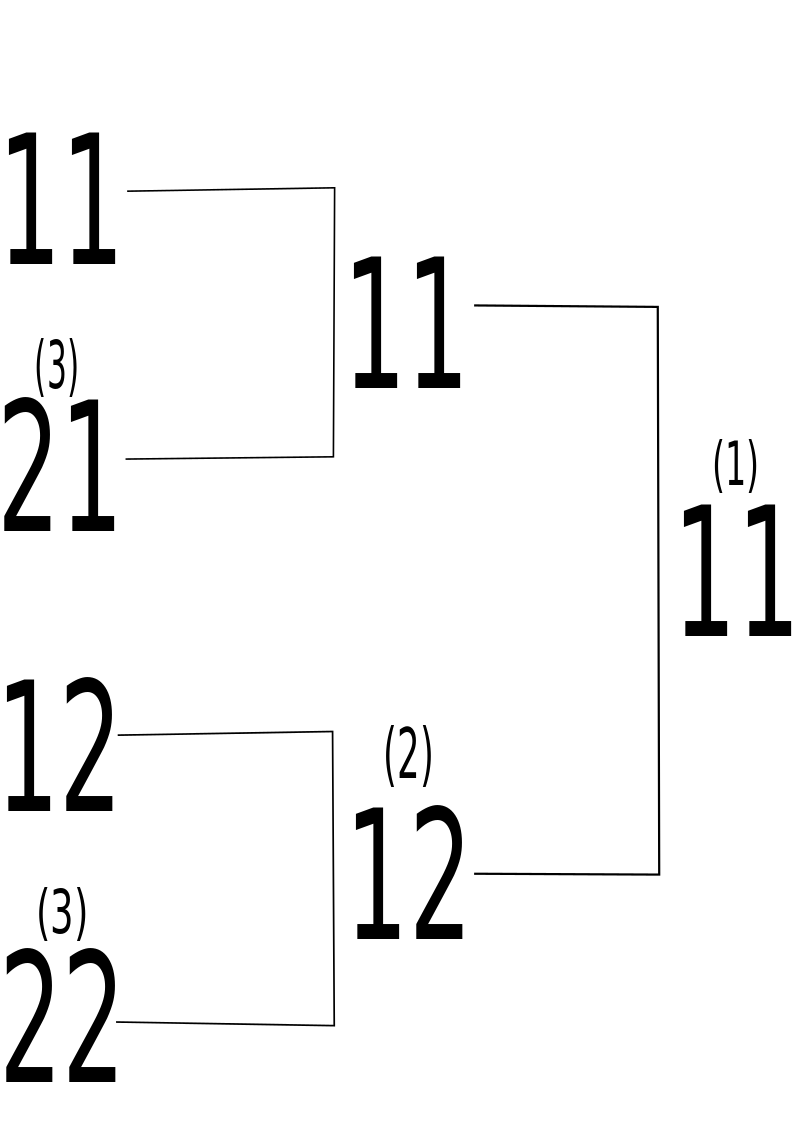
\includegraphics[width=1.75in, height=1.5in]{SimpleTourn.png}
\caption{One possible tournament outcome ranks profile A=11 first, B=12 second, C=21 is ranked third and D=22 fourth.  }
\label{SimpleTourn}
\end{figure}

{\flushleft For} this respondent, profile A=11 is ranked 1 (tournament winner), profile B=10 is ranked 2 (runner-up), profiles C=01 third and D=00 ranked 4. The rationale for the latter 2 rankings is that assuming transitivity in match outcomes, the highest C could be ranked if all profiles were paired is 2, while D could only be ranked as high as 3. Note that there are essentially 24 different possible tournament outcomes, each specifying a ranking or permutation of A,B, C and D.(Table \ref{Tab3}):

\begin{table}[!htpb]
	\scriptsize
	\centering
	\begin{tabular}{c|cccc||cccccc}
		&\multicolumn{4}{c}{Rank}&&\multicolumn{4}{c}{Rank}\\\hline
		Outcome& 1 & 2 & 3&4 &Outcome& 1 & 2 & 3&4  \\\hline
		$O_1$& A&B&C&D&$O_{13}$ &C&A&B&D    \\
		$O_2$& A &B&D&C&$O_{14}$&C&A&D&B     \\
		$O_3$& A&C&B&D&$O_{15}$ &C&B&A&D    \\
		$O_4$& A&C&D&B&$O_{16}$ &C&B&D&A    \\
		$O_5$& A &D&B&C&$O_{17}$ &C&D&A&B    \\
		$O_6$& A&D&C&B&$O_{18}$ &C&D&B&A      \\
		$O_7$& B&A&C&D&$O_{19}$   &D&A&B&C     \\
		$O_8$& B &A&D&C  &$O_{20}$ &D&A&C&B      \\
		$O_9$& B&C&A&D  &$O_{21}$   &D&B&A&C    \\
		$O_{10}$& B&C&D&A  &$O_{22}$ &D&B&C&A   \\
		$O_{11}$& B&D&A&C &$O_{23}$  &D&C&A&B   \\
		$O_{12}$& B&D&C&A &$O_{24}$   &D&C&B&A   \\
	\end{tabular}
	\caption{The 24 possible tournament outcomes or rankings of the profiles A,B,C, and D. Note the lexicographic ordering of these rankings.}
	\label{Tab3}
\end{table}




Each of the $n=4$ sample respondents will have a tournament outcome, which we can compile into an \emph{Individual Ranking Table (IRT)}, an example of which is shown in Table  \ref{Tab1}.
\begin{table}[!htpb]
\centering
\scriptsize
\begin{tabular}{c|cccc|c}
&\multicolumn{4}{c}{Rank}&\\
Respondent& 1 & 2 & 3 & 4&Ranking\\\hline
1& A&B&C&D&$O_1$\\
2& A &C&B&D&$O_3$ \\
3& B &C&A&D& $O_9$ \\
4& A &C&B&D&$O_3$ \\
\end{tabular}
\caption{Profile rankings for a sample of 4 respondents.}
\label{Tab1}
\end{table}
{\flushleft From} this data, it is easy to compute the \emph{Sample Profile Ranking (SPR)} table which indicates how many respondents assigned a particular rank to each profile (Table \ref{SPR}).

\begin{table}[!htpb]
\scriptsize
\centering
\begin{tabular}{c|cccc|c}
&\multicolumn{4}{c}{Rank}&\\
Profile& 1 & 2 & 3&4&SPR\\\hline
A& 3&0&1&0&1.5\\
B& 1 &1&2&0 &2.25\\
C& 0 &3&1&0&2.25 \\
D& 0 &0&0&4&4.0 \\
\end{tabular}
\caption{Sample Profile Ranking (SPR) Table. The $i,j$ entry of the 4x4 matrix forming the body of the table shows the number of respondents who assigned to  the profile in the margin of row $i$, the rank shown by the header in column $j$. The sample profile ranking (SPR) is the arithmetic average of the sample respondent rankings.}
\label{SPR}
\end{table}

Given any profile $X$ and a sample of size $n=4$, the \emph{sample profile ranking (SPR)} $\rho_n(X)=\rho_4(X)$ is obtained as an arithmetic average of the $n=4$ respondents.  For example, for A=11, $\rho_4(A)=[3(1)+1(3)]/4=1.5$, and for C=10 it is $\rho_4(C) = [3(2)+1(3)]/4=2.25$.
In this case, based on the sample, profile A=11 is ranked first, profiles B=10 and C=01 are tied for second, and profile D=00 comes in fourth.

In a similar way, we can use our sample to obtain rankings for each individual attribute level as shown in Table \ref{SAL}.

\begin{table}[!htpb]
	\scriptsize
	\centering
	\begin{tabular}{cc|cccc|c}
		&&\multicolumn{4}{c}{Rank}&\\
		Attribute& Level& 1 & 2 & 3&4&SALR\\\hline
		1& 1 & 4&1&3&0&1.875\\
		1& 0 & 0 &3&1&4 &3.125\\
		2& 1& 3 &3&2&0&1.875 \\
		2& 0 & 1 &1&2&4&3.125 \\
	\end{tabular}
	\caption{Sample Attribute Level Ranking (SAL) Table. }
	\label{SAL}
\end{table}

The main questions we will develop in the sequel are: 
\begin{itemize}
\item POPULATION RANKING INFERENCE \emph{what can we infer from the SRT and SAL tables about the population profile ranking  (PPR) and population attribute level (PAL) tables?}, the latter two meaning the tables for all population respondents; and
\item CHOICE TASK PREDICTION AND ATTRIBUTE IMPORTANCE \emph{for the purpose of choice task predictions and attribute importance rankings, how does information obtainable from the SRT and SAL compare with that obtainable from partworth utilities?}
\end{itemize}

\subsection{A Fundamental Observation}
In this section we explain why  least squares multiple  regression (LSRM) will not in general give exact sample profile rankings. In other words, part-worth utilities can only approximate sample rankings.


\subsubsection{Analytic Approach}

Least squares multiple linear regression (LSRM) can be used to predict sample profile rankings based on individual sample outcomes as we will now explain using our simple 2 attribute, 2 level survey and generic sample data for 4 respondents. Table \ref{Tab7} gives the dataset \{($U_i,V_i,Y_i$)\} ($i = 1,...,16$) where

\begin{eqnarray*}
	U_i&=& 1 \textup{ if attribute 1 has level 1, and 0 if it has level 2}\\
	V_i&=& 1 \textup{ if attribute 2 has level 1, and 0 if it has level 2}\\
	Y_i&=& \textup{ Respondent's ranking of a profile with $U=U_i$, $V=V_i$.}
\end{eqnarray*}

\begin{table}[!htpb]
	\centering
	\small
	\begin{tabular}{cc|ccccc}
		\multicolumn{2}{c}{} &\multicolumn{4}{c}{Output Ranking Data}\\\hline
		$U$ & $V$ & Respondent 1&  Respondent 2& Respondent 3& Respondent 4\\  \hline
		1 &1&$Y_1$&$Y_2$&$Y_3$&$Y_4$\\
		1 &0&$Y_5$&$Y_6$&$Y_7$&$Y_8$ \\
		0 &1&$Y_9$&$Y_{10}$&$Y_{11}$&$Y_{12}$ \\
		0 &0&$Y_{13}$&$Y_{14}$&$Y_{15}$&$Y_{16}$ \\\hline
	\end{tabular}
	\caption{{\small Dataset ranking structure by respondents.}}
	\label{Tab7}
\end{table}


This dataset has certain properties:
\begin{itemize}
	\item
	Each column consists of a respondent's profile rankings, and hence contains the values $1, 2, 3, 4$ in any order.
	
	\item
	Table \ref{Tab7} can also be represented in the form of Table \ref{Tab8}, by which we see that $$\sum U_i = \sum V_i = \sum U_i^2 = \sum V_i^2= 8, $$ and $$ \sum U_iV_i = 4,$$ where the symbol $\sum $ represents $\displaystyle \sum_{n=1}^{16}$.
\end{itemize}


\begin{table}[!htpb]
	\centering
	\small
	\begin{tabular}{cc|c}
		$U$ & $V$ & Rank\\ \hline
		1&	1&	$Y_1$\\
		1&	1&	$Y_2$\\
		1&	1&	$Y_3$\\
		1&	1&	$Y_4$\\
		1&	0&	$Y_5$\\
		1&	0&	$Y_6$\\
		1&	0&	$Y_7$\\
		1&	0&	$Y_8$\\
		0&	1&	$Y_9$\\
		0&	1&	$Y_{10}$\\
		0&	1&	$Y_{11}$\\
		0&	1&	$Y_{12}$\\
		0&	0&	$Y_{13}$\\
		0&	0&	$Y_{14}$\\
		0&	0&	$Y_{15}$\\
		0&	0&	$Y_{16}$\\\hline
	\end{tabular}
	\caption{{\small Dataset's ranking structure with respondents combined.}}
	\label{Tab8}
\end{table}
Using least squares multiple linear regression (LSMR) on the dataset in Table \ref{Tab8}, we estimate each sample profile ranking $Y_i$ as $\hat{Y}_i$:
$$
\hat{Y}_i=c_0 + c_1 U_i + c_2 V_i,
$$
{\flushleft where} the regression coefficients $c_0,c_1,c_2$ are determined by minimizing the sum of squared residuals (SSR):
$$
SSR = \sum_{n=1}^{16}(Y_i-\hat{Y}_i)^2
=\sum_{n=1}^{16}(Y_i-(c_0 + c_1 U_i + c_2 V_i))^2.
$$
To minimize the SSR, we set the partial derivatives with respect to $c_0,c_1$ and $c_2$, equal to zero:
$$\frac{\partial SSR}{\partial c_0} = \frac{\partial SSR}{\partial c_1} = \frac{\partial SSR}{\partial c_2} = 0.$$
This yields the linear system:
$$\begin{cases}
nc_0 +  c_1\sum U_i + c_2\sum V_i = \sum Y_i\\
c_0\sum U_i + c_1\sum U_i^2 + c_2\sum U_iV_i = \sum U_iY_i\\
c_0\sum V_i + c_1\sum U_iV_i + c_2\sum V_i^2 = \sum V_iY_i
\end{cases},$$\\
which is equivalent to the matrix equation:

\[
\begin{bmatrix}
n& \sum U_i& \sum V_i \\
\sum U_i&\sum U_i^2&\sum U_iV_i\\
\sum V_i& \sum U_iV_i& \sum V_i^2\\

\end{bmatrix}
%
\begin{bmatrix}
c_0 \\
c_1\\
c_2
\end{bmatrix}
=
\begin{bmatrix}
\sum Y_i\\
\sum U_iY_i\\
\sum V_iY_i
\end{bmatrix}
.
\]

{\flushleft Simplifying} the sums and using Cramer's Rule  we obtain the regression coefficients $c_0,c_1$ and $c_2$:

$$
c_0 =
\frac{
	\begin{bmatrix}
	\sum Y_i & 8 & 8\\
	\sum U_iY_i& 8 & 4\\
	\sum V_iY_i & 4 & 8
	\end{bmatrix}
}{256} = \frac{
	\begin{bmatrix}
	\sum Y_i & 2 & 2\\
	\sum U_iY_i& 2 & 1\\
	\sum V_iY_i & 1 & 2
	\end{bmatrix}
}{16},
$$
$$
c_1 =
\frac{
	\begin{bmatrix}
	16 & \sum Y_i & 8 \\
	8 & \sum U_iY_i& 4\\
	8 & \sum V_iY_i & 8
	\end{bmatrix}
}{256} = \frac{
	\begin{bmatrix}
	4 & \sum Y_i & 2 \\
	2 & \sum U_iY_i& 1\\
	2 & \sum V_iY_i & 2
	\end{bmatrix}
}{16}, \textup{and}
$$
$$
c_2 =
\frac{
	\begin{bmatrix}
	16 &  8 & \sum Y_i\\
	8 & 8 & \sum U_iY_i \\
	8 & 4 & \sum V_iY_i
	\end{bmatrix}
}{256} = \frac{
	\begin{bmatrix}
	4 & 2 & \sum Y_i\\
	2 & 2 & \sum U_iY_i \\
	2 & 1 & \sum V_iY_i
	\end{bmatrix}
}{16}.
$$

The LSMR predicted profile rankings $ \hat{Y}_{uv}$  are given by:
$$\hat{Y}_{11} = c_0 + c_1 + c_2 =
\frac{2\sum U_iY_i + 2\sum V_iY_i - \sum Y_i}{16},$$
$$\hat{Y}_{10} = c_0 + c_1 =
\frac{-6 \sum V_iY_i + \sum U_iY_i + \sum Y_i}{16},$$
$$\hat{Y}_{01} = c_0 + c_2 =
\frac{-2\sum U_iY_i + 2\sum V_iY_i + \sum Y_i}{16}, \textup{  and}$$
$$\hat{Y}_{00} = c_0 =
\frac{-2\sum U_iY_i - 2\sum V_iY_i +3 \sum Y_i}{16}.$$
The corresponding actual sample profile rankings obtained by averaging the respondent rankings are:
$$\bar{Y}_{11} = \frac{Y_1+Y_2+Y_3+Y_4}{4},$$
$$\bar{Y}_{10} = \frac{Y_5+Y_6+Y_7+Y_8}{4},$$
$$\bar{Y}_{01} = \frac{Y_9+Y_{10}+Y_{11}+Y_{12}}{4}, \textup{  and}$$
$$\bar{Y}_{00} = \frac{Y_{13}+Y_{14}+Y_{15}+Y_{16}}{4}.$$


{\flushleft We} thus have the following theorem: \emph{The sample profiles' LSMR predicted and actual rankings are the same if and only if the following four equations hold}
\begin{equation}
\textup{(profile 11)} :  2\sum U_iY_i + 2\sum V_iY_i - \sum Y_i = 4( Y_1+Y_2+Y_3+Y_4 ),
\end{equation}
\label{eq:14}
\begin{equation}
\textup{(profile 10)} :  -6 \sum V_iY_i + \sum U_iY_i + \sum Y_i = 4( Y_5+Y_6+Y_7+Y_8 ),
\end{equation}
\label{eq:15}
\begin{equation}
\textup{(profile 01)} : -2\sum U_iY_i + 2\sum V_iY_i + \sum Y_i = 4(Y_9+Y_{10}+Y_{11}+Y_{12} ), \textup{and}
\end{equation}
\label{eq:16}
\begin{equation}
\textup{(profile 00)} : -2\sum U_iY_i - 2\sum V_iY_i +3 \sum Y_i = 4(Y_{13}+Y_{14}+Y_{15}+Y_{16} ).
\end{equation}
\label{eq:17}

{\flushleft Furthermore}, by adding these equations, we obtain a corollary:
\emph{The following is a necessary condition for the LSMR predicted sample profile rankings to equal the sample profile rankings:}
\begin{equation}
\sum U_iY_i = \sum V_iY_i.
\label{cor}
\end{equation}


Returning to our small sample (Table \ref{Tab1}), we see that the average profile rankings and LSRM predicted profile rankings are different for each of the four profiles (Table \ref{Tab9}). In this case, the regression coefficients are
$c_0=3.75$, $c_1=-1.25$, $c_2=-1.25$.  The equality (\ref{cor}) in the corollary does not hold.


\begin{table}[!htpb]
	\centering
	\scriptsize
	\begin{tabular}{cc|cccc|c|c|c}
		\multicolumn{2}{c}{} &\multicolumn{4}{c}{Respondents}\\\hline
		$U$ & $V$ & R 1&  R 2& R 3& R 4 &Sample Rank&Predicted Sample Rank& $\mid$Residual Error$|$\\  \hline
		1 &1&1&1&3&1&1.5&3.75-1.25(1)-1.25(1)=1.25&.25\\
		1 &0&2&3&1&3&2.25&3.75-1.25(1)-1.25(0)=2.5&.25 \\
		0 &1&3&2&2&2&2.25 &3.75-1.25(0)-1.25(1)=2.5&.25 \\
		0 &0&4&4&4&4&4 &3.75-1.25(0)-1.25(0)=3.75&.25\\\hline
	\end{tabular}
	\caption{{\small Predicted rankings for the sample outcomes in Table \ref{Tab1}.}}
	\label{Tab9}
\end{table}



The conditions  (12)-(15) for whether or not the LSMR  profile ranking predictions are error-free may be understood geometrically by considering points in an $x_1x_2x_3$ coordinate system in which the $x_1x_2$ coordinates represent the profile and the $x_3$ coordinate the ranking. For our simple generic survey,  if the four points representing the sample profile rankings are co-planar, there is no error; otherwise, the LSMR predicted profile rankings will have a residual error (Figure  \ref{sec4fig}).  Such a geometric interpretation  is not possible for surveys involving more than 2 attributes, in which case standard LSMR residual analysis indicates the error in sample  profile rankings using regression coefficients.


\begin{figure}[!htpb]
	\centering
	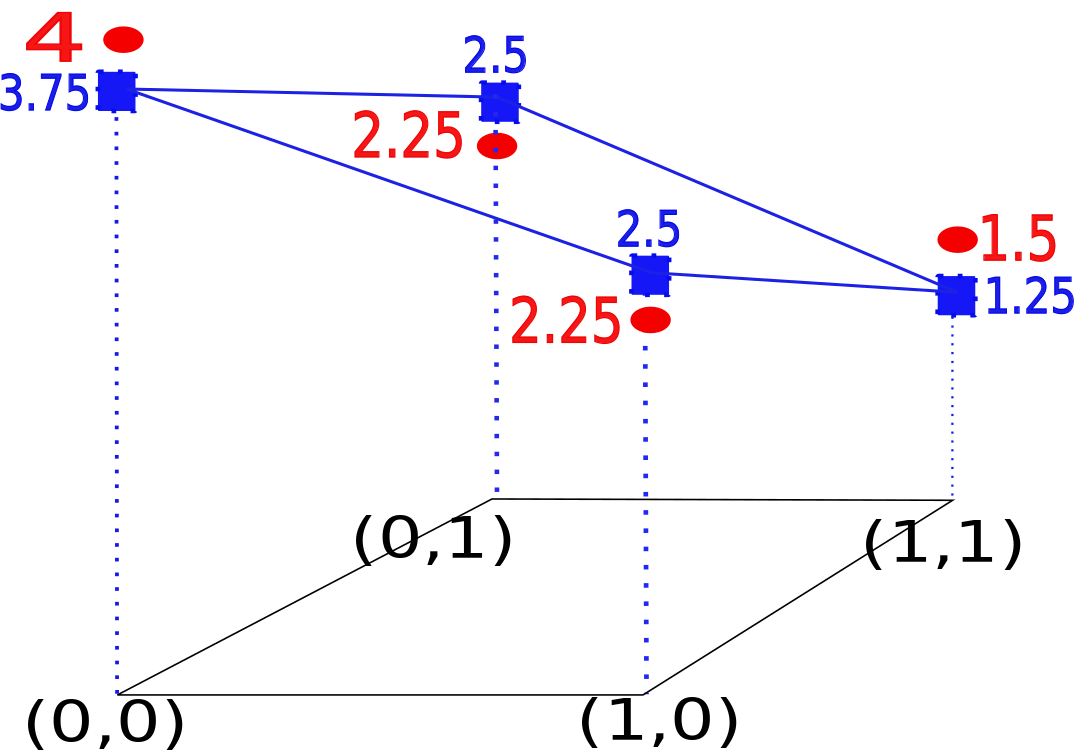
\includegraphics[width=2in,height=2in]{sec4fig.png}
	\caption{{\small The LSRM predicted sample profile rankings ($\hat{Y}_{ij}=3.75-1.25U_i-1.25V_j$ (square vertices) have residual errors as the actual sample rankings (dots) do not belong to the plane of regression. }}	
	\label{sec4fig}
\end{figure}


\subsection{Maximum Likelihood Estimation of the PRT}
We will proceed to develop PR-ACBC methodology without assuming any knowledge of partworth utilitites.  
\subsubsection{Known Population Size}
Let us assume the population has size $N=7$, and that our sample was a random selection of 4 out of these 7. The number $N=7$ is for simplicity of illustrating the relevant conmputations only, and could be any number $N>n=4$.  We will now use a multivariate hypergeometric distribution to obtain the maximum likelihood estimate (MLE) PPR, meaning the population which was must likely to have yielded the observed sample outcomes.  

To begin, we create what we shall call a \emph{factor table} (Table \ref{FT}) 
\begin{table}[!htpb]
	\scriptsize
	\centering
	\begin{tabular}{r|ccc|c}\hline
		\multicolumn{5}{c}{Choose the $k=3$ largest factors $f_{ij}$ for a population size $N=n+k=n+3$.}\\ 
		+3& $f_{13}=4/3$ & $f_{23}=5/3$&$f_{33}=4/3$&\\
		+2& $f_{12}=3/2$ & $f_{22}=2$ &$f_{32}=3/2 $&\\
		+1& $f_{11}=2$  &$f_{21}=3$&$f_{31}=2 $ &\\\hline
		Number observed in sample:&$n_1=1$& $n_2=2$ & $n_3=1$ & Sample size: $n=4$\\\hline
		Ranking:&1=$O_1$&2=$O_3$&3=$O_9$
	\end{tabular}
	\caption{Probability factor table. The $k=3$ largest factors $f_{ij}=1+(n_i/j)$ are used to determine the MLE PRT for a population size $N=n+k=4+3=7$. }
	\label{FT}
\end{table}
{\flushleft  Let} $N_j$ denote the number of rankings $O_j$ in the PRT.  The number of factors $a_j$ chosen from column $j$ indicates that a  PRT with $N_j= n_j+a_j$ is a MLE.    In our case, the latter is not unique.  One choice of 3 largest factors is $f_{11}=2, f_{21}=3,f_{22}=2$ so that $a_1=1$, $a_2=2$ and $a_3=0$. A population $Y$ in which $N_1=n_1+a_1=2$ , $N_2=n_2+a_2=4$, and $N_3=n_3+a_3=1$ is a MLE. Another choice of 3 largest factors  is $f_{11}=2, f_{21}=3,f_{31}=1$ so that $a_1=1$, $a_2=1$ and $a_3=0$. Population $Z$ in which $N_1=n_1+a_1=2$ , $N_2=n_2+a_2=3$, and $N_3=n_3+a_3=2$ is also MLE. We can verify this is so by computing the respective probabilities $p_Y$ and $p_Z$ that our observed sample arises from erspective populations $Y$ and $Z$ :

\begin{equation}
p_Y=\frac{C(2,1)C(4,2)C(1,1)}{C(7,4)}=\frac{f_{11} \cdot f_{21}f_{22}}{C(7,4)}
\end{equation}
{\flushleft and }
\begin{equation}
p_Z=\frac{C(2,1)C(3,2)C(2,1)}{C(7,4)}=\frac{f_{11}\cdot f_{21}\cdot f_{31}}{C(7,4).}
\end{equation}
{\flushleft This} procedure generalizes to any number of rankings $m$ which appear in a sample of sample $n$ ( Oberhofer and Kaufman (1987)). Let $n=\sum_{j=1}^m n_j$ where $n_j$ is the number of ranking $j$ appearing in the sample.  Form the probability factor table with $f_{ij}=1+\frac{n_i}{j}$ ($i=1,...,r$, $j=1,...,m$ and $N=n+r$.)  Choose the $r$ largest factors in the latter table and let $a_j$ be the number of factors chosen in column $j$.  Then a population with a PRT such  $N_j=n_j+a_j$ ($j=1,...,m$) is a MLE. 
\subsubsection{Unknown Population Size}


Let us assume now that rather than having a specified size, the population size is an unknown value $N$.  In this case, we wish to determine the probability $p_i$  that a member of the population has ranking $O_i$.  As before, we assume that our sample is drawn randomly from the population. The probability $p$ that the observed sample consisting of one $O_1$, two $O_3$'s and one $O_9$ is

\begin{equation}
p=f(p_1,p_3,p_9)=\frac{4!}{1!2!1!}[p_1p_3^2p_9],
\end{equation}
\label{eq:1}
{\flushleft where} $g(p_1,p_3,p_9)=p_1+p_3+p_9=1$.
The values of $p_1^*,p_3^*,$ and $p_9^*$ which maximize $H(p_1,p_3,p_9)=\ln (f(p_1,p_3,p_9))$ (and hence also maximizes $p=f(p_1,p_3,p_9)$)  are obtained using Lagrange multipliers:
\begin{eqnarray*}
	\nabla H(p_1^*,p_3^*,p_9^*) & = & \lambda \nabla g
	(p_1^*,p_3^*,p_9^*),
\end{eqnarray*}
{\flushleft and therefore}
\begin{eqnarray*}
	\frac{1}{p_1^*} & = & \lambda\\
	\frac{2}{p_23^*} & = & \lambda\\
	\frac{1}{p_9^*} & = & \lambda.
\end{eqnarray*}
{\flushleft (The scalar quantity $\lambda$ is called a Lagrange multiplier.) Using} $p_1^*+p_3^*+p_9^*=1$ gives $\frac{1}{\lambda} + \frac{2}{\lambda}+\frac{1}{\lambda}=1$ and so $ \lambda = 4$.  Hence, the values $p_1^*=\frac{1}{4}, p32^*=\frac{1}{2}$, $p_9^*=\frac{1}{4}$ maximize the probability of the observed sample outcomes.  

In general, let $n_k$ be the number of sample outcomes $O_k$ ($k=1,2,...,K$) and let $p_k$ be the probability that a respondent in the population  has outcome $O_k$ $(k= 1, 2, ..., K)$.  The likelihood function $f(p_1, p_2, ..., p_K)$ giving the probability of observing the sample values $n_1, ..., n_{K}$ is given by

\begin{equation}
f(p_1, ...., p_K)= \frac{n!}{n_1!n_2!\cdot\cdot\cdot n_K!} \prod_{k=1}^K p_k^{n_k},
\end{equation}
\label{eq:4}

{\flushleft with} $\sum_{k=1}^{K}n_k=n$ and $\sum_{k=1}^{K}p_k=1$.
We seek to find the values $p_1^*, ..., p_{K}^*$ which maximize the likelihood function $f$, or equivalently, the log-likelihood function

\begin{equation}
H(p_1, ..., p_K)=\ln f = \ln(n!) - \sum_{k=1}^{K} n_k! +\sum_{k=1}^{K} n_k\ln(p_k),
\end{equation}
\label{eq:5}
{\flushleft subject} to the constraint $g(p_1, ..., p_{K})=p_1+p_2+...+p_K=1$.  Properties of gradients imply that the optimal values $p_i^*$ must satisfy

\begin{equation}
\nabla H(p_1^*, ..., p_K^*) = \lambda \nabla g(p_1^*, ..., p_{K}^*).
\end{equation}
\label{eq:6}
{\flushleft It} follows that for $k=1, ..., K$,

\begin{equation}
\frac{n_k}{p_k^*}=\lambda.
\end{equation}
\label{eq:7}
{\flushleft Hence,} $n=\sum_{k=1}^{K} n_k =  \lambda \sum_{k=1}^{K} p_k^* = \lambda$, and so the probabilities $p_k^* = \frac{n_k}{n}$ give the maximum likelihood of the observed sample outcomes $n_k$ ($k=1, 2, ..., K$).  For any sample of size $n$ and number $n_k$ of observed outcomes $O_k$ ($k=1, 2, ...K$), the maximum likelihood probabilities $p_k^*=\frac{n_k}{n}$
indicate that for a population of size $N$, the expected number $N_k$ of outcomes $O_k$ is given by $E(N_k)=p_k N.$  A maximum-likelihood population could be simulated by augmenting the observed $n$ sample outcomes, where the probability of outcome $O_k$ at each draw is given by $p_k$.   For a large number of such randomly constructed populations of size $N$, for each $k$ the average number of population outcomes $O_k$ is approximately $p_k N$.






\subsection{Population Ranking Intervals}

Maximum likelihood  provides a point estimate into the population profile rankings, meaning the PRT most likely to have produced the observed sample. In this section, given ranking data for a sample consisting of $n$ survey respondents selected at random from a population with $N> n$ respondents, we will show how to construct for each profile ranking intervals   which are guaranteed to include the population profile rankings.

\subsection{Population Ranking Range}

Returning to our simple example, in which each profile is ranked 1, 2, 3 or 4, let $\rho_k(X)$ denote the ranking of profile $X$ based on tournament results for $k$ respondents. Note that for any population of $k$ respondents ($n\le k \le N$) which contains an observed sample of size $n$, the following inequality must hold:

\begin{equation}
\frac{k+n(\rho_n(X)-1)}{k}\le \rho_k(X)  \le \frac{3k+n(\rho_n(X)-3)}{k}.
\label{eq6}
\end{equation}

{\flushleft This} interval containing $\rho_k(X) $ is obtained by either (i) assigning the  rank 1 to $X$ for all $k-n$ members of the population not in the sample (lower bound for $\rho_k(X)$); or (ii) assigning the rank 3 to $X$  for all $k-n$ non-sample population members (upper bound for $\rho_k(X)$). Taking $k=N$, a sample of size $n$ provides  a 100\% confidence interval $$\frac{N+n(\rho_n(X)-1)}{N}\le \rho_N(X)  \le \frac{3N+n(\rho_n(X)-3)}{N}$$ for the population ranking $\rho_N(X)$ of any profile $X$.

Insight into the confidence interval (\ref{eq6}) is gained when we write it in the form

\begin{equation}
\rho_n(X)-e_1 \le \rho_k(X) \le \rho_n(X)+e_3,
\end{equation}
\label{eq:9}

{\flushleft where} $e_1$ is the maximum distance from $\rho_k(X)$ to $\rho_n(X)$ towards the lower ranking bound 1, and $e_3$ is the maximum distance  from $\rho_k(X)$ to $\rho_n(X)$ towards the upper ranking bound 3. Note further that


\begin{equation}
\frac{k+n(\rho_n(X)-1)}{k} = \rho_n(X)-e_1,
\end{equation}
\label{eq:10}
{\flushleft which implies}

\begin{equation}
e_1 = \frac{k-n}{k}(\rho_n(X)-1).
\end{equation}
\label{eq:11}
{\flushleft Similarly,}

\begin{equation}
\frac{3k+n(\rho_n(X)-3)}{k} = \rho_n(X)+e_2,
\end{equation}
\label{eq:12}
{\flushleft which} yields

\begin{equation}
e_2=\frac{k-n}{k}(3-\rho_n(X)).
\end{equation}
\label{eq:13}
{\flushleft Let} $\lambda=\frac{k-n}{k}$ be the proportion of the population which has not taken the survey. In both directions, the interval extends from $\rho_n(X)$ a distance $\lambda$ times the distance to the endpoints of the ranking interval $[1, 3]$. In addition, the length of this confidence interval is given by  $e_1+e_2=2\lambda$, as seen in Figure \ref{AL}. Note that the coefficient 2 of $\lambda$ arises algebraically as the difference between  the extreme rankings 1 and 3.

\begin{figure}[!htpb]
\centering
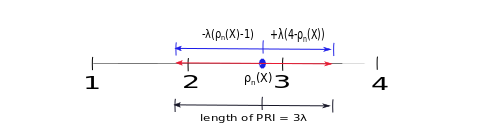
\includegraphics[width=6.5in, height=1.75in]{Confidence_Interval.png}
\caption{Given a profile $X$ and its sample ranking $\rho_n(X)$, a 100\% confidence interval for the population profile ranking $p_k(X)$ is determined by $\lambda=\frac{k-n}{k}$, the proportion of the population who have not taken the survey.}
\label{AL}
\end{figure}


\subsection{Application}

These results can be used to quantify the possible consequences of survey response bias. For the simple example introduced in Section 2, let us consider the following response scenarios. Assume that, out of the total population $N=8$, two respondents have outright refused to take the survey, four have completed it, and the other two have not yet replied. If the analysis is performed with only the sample of $n=4$ respondents, then the length of the confidence interval is  $\frac{2(8-4)}{8}=1$. If one of the non-respondents is convinced to participate, the interval length is reduced to $\frac{2(8-5)}{8}=\frac{3}{4}$, improving the precision by 25\%. If both of the non-respondents participate, then the interval is further reduced to $\frac{2(8-6)}{8}=\frac{1}{2}$. In other words, the two non-respondents  cause the confidence interval to be twice as large, an important consideration in seeking to elicit survey response.

\subsection{Attribute Decomposition Via 2 Dimensional Multimensional Scaling}
\subsection{Application: Profile Ranking Analysis of a Small Population Disaster Relief Survey}


In this section we show how to apply PR ACBC methodology to an actual survey.

\section{ACBC Survey of Humanitarian Disaster Relief Organizations}

PR-based ACBC methodology for analyzing small populations has many possible applications. In disaster relief, effectiveness of a response may depend on the quality of collaboration between organizations with a broad diversity of religious and ideological perspectives. For effective coordination of relief, it is important that humanitarian organizations understand the unique traits and characteristics that shape their disaster response decisions. Through comparison of these factors, it is possible to design optimal partnerships and joint endeavors between organizations that may fulfill distinct, yet complimentary, humanitarian roles. Our research focused on how faith based organizations (FBOs) prioritize key attributes affecting their decision whether or not to respond to an international humanitarian disaster.

To this end, we designed a survey that creates "Go/No-Go" decision profile preferences for a small population of approximately 50 international FBOs with headquarters in the United States. The attributes and levels for this survey are displayed in Figure \ref{AL}. Different disaster scenarios face off against each other in the tournament stage and are given rankings based on their performance. The purpose of the ranking is to determine whether FBOs fill a certain niche in disaster response landscape as might be inferred for by their ``number-one'' or ``top-three'' ranked disaster response profiles. As a case study, we discus how our methodology was applied to data obtained for this survey administered using Sawtooth's Lighthouse platform.

\begin{figure}[!htpb]
\centering
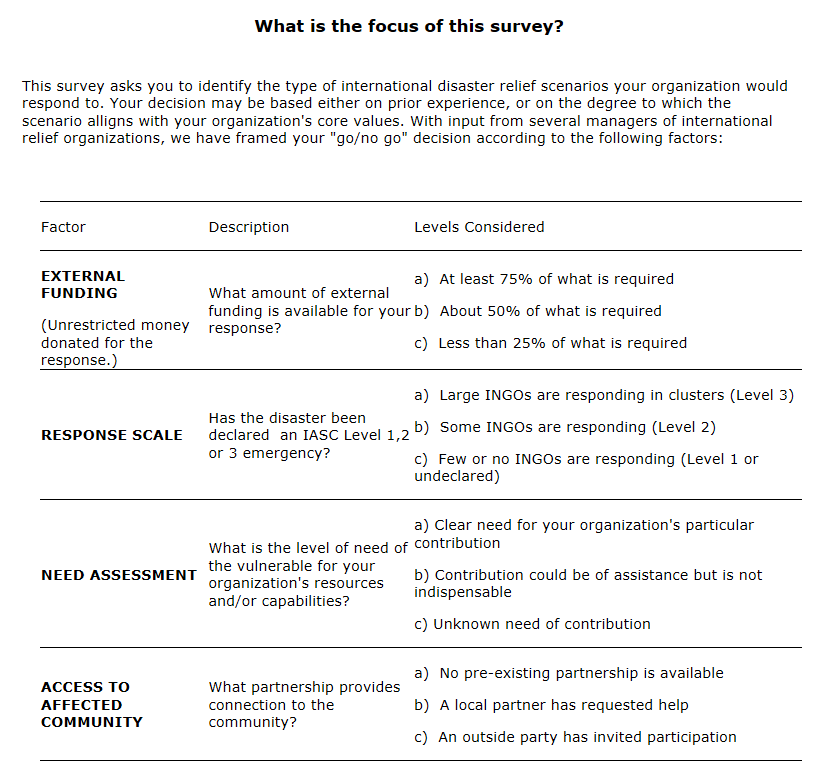
\includegraphics[width=5.75in, height=7in]{AttributeLevels.png}
\caption{{\small An ACBC survey with 4 attributes consisting of 3 levels each. }}
\label{AL}
\end{figure}



\subsection{Ranking Method}

As shown in Figure 4, our humanitarian survey consists of four attributes, each with three levels. Thus, the number of possible profiles is $3^4=81$. These are identified by four digit numbers $X=x_1x_2x_3x_4$ where profile $X$ has level $x_1$ for the first attribute, level $x_2$ for the second attribute, level $x_3$ for the third attribute, and level $x_4$ for the fourth attribute. In the tournament stage of the competition, there are four rounds, in which sixteen profiles face off against each other in head to head match-ups, much like the FIFA World Cup Round of 16. The competing profiles are selected from the 81 possible profiles based on the respondent's BYO preferences. We assign a ranking of 1 to the tournament winner, 2 to the runner up, 3 to the semifinal losers, 4 to the quarterfinal losers, 5 to the profiles that are eliminated in the first round, and 6 to those that do not appear in the tournament. By the two-week deadline after deploying the survey, 5 FBOs had responded, resulting in the sample ranking table shown in Table \ref{Tab13}. The responding population ($N=10$) most likely to produce this observed sample is also included.

\begin{table}[!htpb]
\scriptsize
\centering
\begin{tabular}{c|ccccc|ccccc|ccc|c}
Profile& 1 & 2 & 3 & 4 & 5 & 6&7&8&9&10&11&12&13&PR\\\hline
1212& 2&	3&	7&	3&	7&	7&	1&	7&	7&	7&	4&	1&	7&	4.846\\
1112&7	&1	&7	&7	&1	&2	&7	&5	&7	&3	&7	&7	&4	&5.000\\
1312&7	&7	&7	&7	&5	&5	&7	&1	&1	&1	&7	&7	&3	&5.000\\
3212&7	&7	&7	&5	&5	&1	&2	&7	&4	&7	&7	&7	&1	&5.154\\
1122&1	&7	&7	&4	&7	&7	&5	&7	&4	&7	&3	&3	&7	&5.308\\
2212&7	&5	&5	&7	&7	&7	&7	&2	&7	&4	&2	&2	&7	&5.308\\
1222&7	&7	&4	&7	&4	&5	&7	&4	&3	&2	&7	&7	&7	&5.462\\
1232&5	&7	&7	&5	&5	&5	&4	&5	&7	&5	&7	&7	&2	&5.462\\
2312&7	&7	&7	&1	&5	&3	&4	&7	&2	&7	&7	&7	&7	&5.462\\
2112&3	&7	&7	&4	&5	&4	&3	&7	&7	&7	&7	&7	&5	&5.615\\\hline
\end{tabular}
\caption{{\small Top 10 ranked profiles for FBOs ($n=13,N=50$) }   }
\label{Tab13}
\end{table}


\subsection{Profile Rank Confidence Intervals}

Applying the results of Section 3, using the data in Table \ref{Tab13}, given a profile's sample ranking ($n=5$), we can construct confidence intervals for  population rankings with $N=10$. For example, consider the  profile 1232 which had the top ranking in the sample.  In a population with $N=10$ and $\rho_n(1232)=4.2$, the value $\lambda=\frac{1}{2}$ results in the confidence interval shown in Figure \ref{fig:4}. Since the range of individual rankings is $6-1=5$, we compute the interval length as $5\lambda = 2.5$. It follows that that the population ranking $\rho_k(2113)$ could be up to 1.6 less or .9 greater than the sample ranking $\rho_5(1232)=4.2$. After following up with organizations to whom we sent the survey, we received survey data from an additional 5 FBOs, and calculated $\rho_{10}(1232)=4.6$, which falls within our confidence interval (Figure \ref{fig:4}). This approach can be applied to any profile in Table \ref{Tab13} and provides a simple visualization  of the extent to which sample profile rankings can capture population profile rankings.


\begin{figure}[!htpb]
\centering
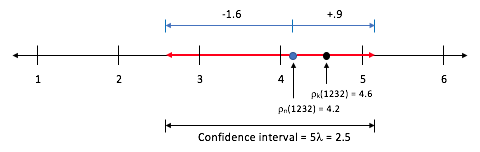
\includegraphics[width=5.75in, height=2.75in]{Confidence_Interval_2.png}
\caption{Confidence Interval for profile 1232 (n = 5, k = 10).}
\label{fig:4}
\end{figure}

\subsection{Visualization of Top Ranked Profiles}
A final outcome of PR ACBC would be a visual representation of the top ranked profiles. For the population rankings in Table \ref{Table 13}, there is a triple tie for the number 1 ranking.  A visual display of top-ranked profiles such as shown in Figure \ref{fig:6}, might enhance the GUI of existing ACBC software.

\begin{figure}[!htpb]
\centering
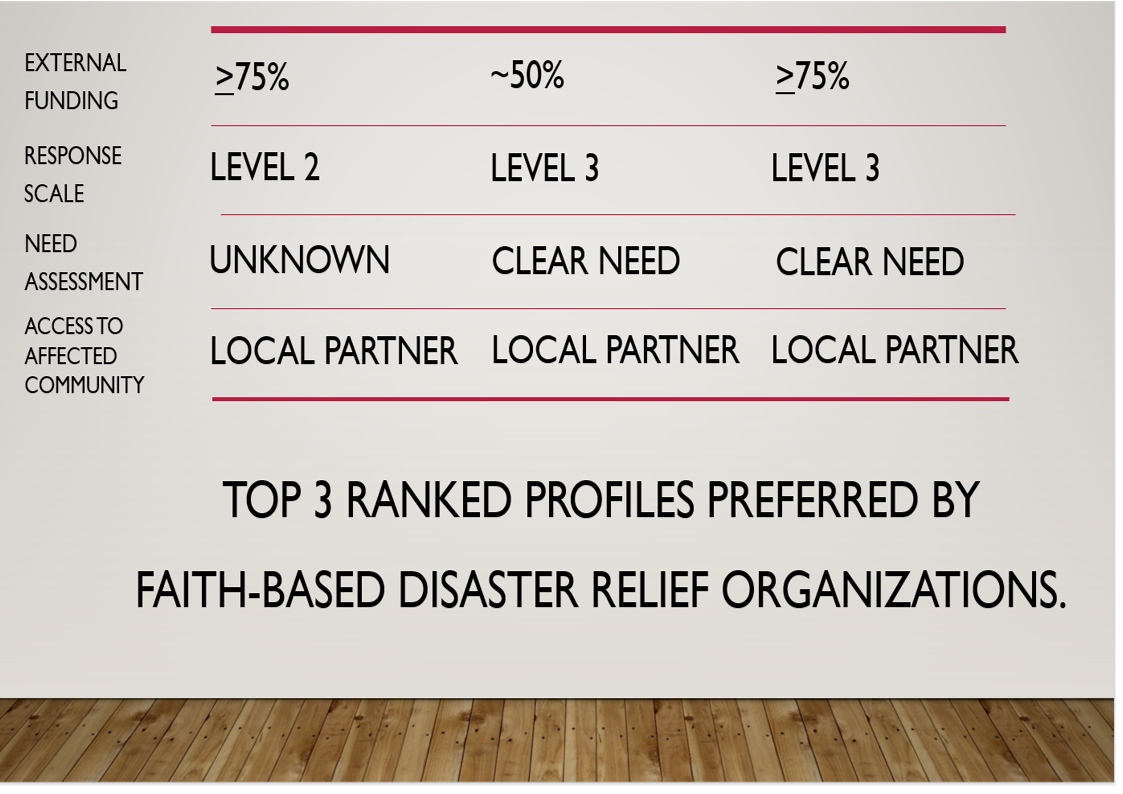
\includegraphics[width=5.75in, height=2.75in]{Fig6.png}
\caption{A visual lineup of top-ranked profiles could enhance the GUI of commercial ACBC software.}
\label{fig:6}
\end{figure}





\section{Conclusion}
Unlike conjoint analysis of survey data where the target populations are large and more suitable for conventional statistical tools, we have introduced a simple, intuitive approach to a small population's profile rankings based on sample data. The population most likely to yield the given sample results are expected to have the same profile rankings as the sample's. We also provide a new type of 100\% confidence interval for profile rankings without using standard deviations, which can be used to quantify maximum possible survey response bias. Furthermore, we have shown that part-worth utilities obtained by multiple linear regression can only replicate sample profile rankings under special conditions, with the residuals indicating the errors in predicted rankings.

For applications such as humanitarian disaster relief, sample profile ranks are more easily understandable to respondents than part-worth utilities. The intuitive nature of profile ranking allows quick and straightforward analysis of any small sample of disaster response organizations. Given that the sample  comprises a relatively significant portion of the overall population, 100$\%$ confidence intervals provide an absolute range of possible population profile rankings without the complexity of statistical inference. Consequently, for small organizations with low operating costs, these techniques may serve as an effective, yet affordable, alternative to more sophisticated ACBC survey utility-based analysis software. Moreover, a visualization of top-ranked or bottom-ranked profiles is a good way to summarize PR ACBC survey results.

Major areas open to further research include analysis of  different ranking systems for various types of choice tournaments and application of PR ACBC methodology to other small population studies.



\subsection*{Acknowledgements}

The authors would like to thank
Erica Gralla, Jarrod Goenzel, Timotius Kartawijaya, and Mike Veatch for their valuable contributions to this work.


\section*{References}
\begin{list}{}{\itemindent=-2em}
\small
\item Alvo, M., and Yu, P.L.H. 2014. \emph{Statistical Methods for Ranking Data}. Springer.

\item Gralla, E., Goentzel, J., and Fine G. 2014. Assessing trade-offs among multiple objectives for humanitarian aid delivery using expert preferences.
\emph{Production and Operations Management}, Springer-Verlag Berlin 23(6), 978-989.

\item Oberhofer, W. and Kaufman, H.1987.  Maximum Likelihood Estimation of a Multivariate Hypergeometric Distribution. \emph{Sankhya: The Indian Journal of Statistics, Series B (1960-2002)}, Indian Statistical Institute, 49(2), 188-191. 

\item Orme, B.K., and Chrzan, K. 2017. \emph{Becoming an Expert in Conjoint Analysis: Choice Modeling for Pros.} Sawtooth Software.

\item Rao, V. R. 2014. \emph{Applied Conjoint Analysis}. Springer.

\item  Stewart, J. 2016.  \emph{Calculus, Early Transcendentals (8E)}. Cengage Learning.

\item Rossi, P., Allenby, G. and McCulloch R. 2005. \emph{Baysian Statistics and Marketing.} John Wiley \& Sons, Ltd.


\end{list}
\end{document}
